\documentclass{beamer}
\usepackage[utf8]{inputenc}   % caracteres especiales (acentos, eñes)
\usepackage[spanish]{babel}     % varias definiciones para el español

\mode<presentation> {
\usetheme{Madrid}
}

\usepackage{graphicx} % Allows including images
\usepackage{booktabs} % Allows the use of \toprule, \midrule and \bottomrule in tables

\title[Clasificador por géneros musicales]{Clasificador de canciones según géneros musicales} 

\author[Fagioli, Matzkin, Oberti]{Gianfranco Fagioli,
		Victor Matzkin,
		Gaspar Oberti}
		
\institute[FICH-UNL]
{
Procesamiento Digital de Señales\\
Facultad de Ingeniería y Ciencias Hídricas\\
Universidad Nacional del Litoral
\medskip
}
\date{\empty}

\begin{document}

\begin{frame}
\titlepage % Print the title page as the first slide
\end{frame}

\begin{frame}
\frametitle{Contenidos}
\tableofcontents 

\end{frame}

\section{Introducción}

\subsection{Géneros musicales}

\begin{frame}

\frametitle{Definiciones}

\begin{block}{Género}
Forma de categorizar a las canciones a partir de una determinada percepción del ser humano.
\end{block}

\begin{block}{Clasificador de géneros}
Distinguir entre géneros utilizando características propias de la señal, que se pueden obtener a partir de mediciones en el dominio temporal y frecuencial. Haciendo uso de un clasificador estadístico, luego se procede a estimar el género de un conjunto de canciones.
\end{block}

\end{frame}


\section{Extracción de Características}

\begin{frame}

\begin{block}{Extracción de Características}
Caracterizar un segmento de audio mediante una representación numérica compacta. Se extraerán dos tipos de características: de timbre y de ritmo.
\end{block}

\end{frame}

\subsection{Características del Timbre}
\begin{frame}

\begin{block}{Timbre}
El timbre es una de las cuatro cualidades que caracteriza al sonido, y es el que nos permite diferenciar dos sonidos de igual frecuencia fundamental e intensidad (por ejemplo, la misma nota tocada con dos instrumentos diferentes). 
\end{block}

\begin{itemize}
\item Análisis de Fourier
\item Tamaño de la ventana
\item Textura del timbre
\item Media y varianza de características
\end{itemize}

\end{frame}

\begin{frame}
\frametitle{Centroide espectral}

\begin{itemize}
\item Centro de masa del espectro
\item \textit{Brillo} del sonido
\end{itemize}

$$C_t = \dfrac{\sum_{n=1}^{N} M_t[n] * n}{\sum_{n=1}^{N} M_t[n]}$$

\end{frame}

\begin{frame}
\frametitle{Roloff espectral}
\begin{itemize}
\item Concentración de energía
\end{itemize}
$$C_t = \sum_{n=1}^{R_t} M_t[n] = 0.85 * \sum_{n=1}^{N} M_t[n] $$
\end{frame}

\begin{frame}
\frametitle{Flujo espectral}
\begin{itemize}
\item Cuánto cambia la potencia del espectro de una ventana a otra.
\item Norma-2.
\end{itemize}
$$F_t  = \sum_{n=1}^{N} (N_t[n]-N_{t-1}[n])^2$$
\end{frame}

\begin{frame}
\frametitle{Cruces por cero en el dominio del tiempo}
\begin{itemize}
\item Medida del ruido de la señal.
\end{itemize}

$$Z_t = \frac{1}{2} \sum_{n=1}^{N} |signo(x[n]) - signo(x[n-1])|$$ 

\end{frame}

\begin{frame}
\frametitle{Coeficientes cepstrales en la escala de Mel (MFCC)}
\begin{itemize}
\item Cepstrum.
\item Banco de filtros (5 primeros coeficientes).
\begin{center}
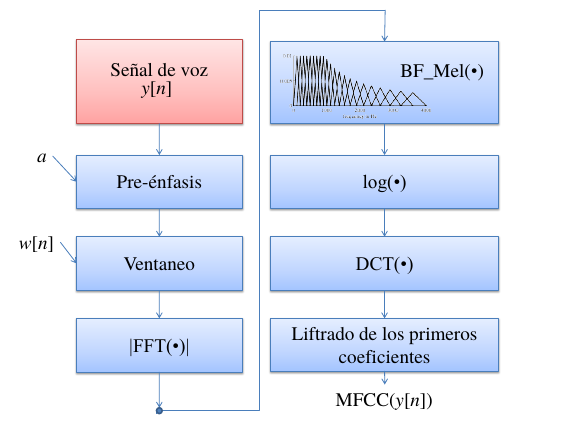
\includegraphics[width=0.7\linewidth]{mfcc}
\end{center}
\end{itemize}

\subsection{Características del Ritmo}

\end{frame}

\begin{frame}
\begin{block}{Ritmo}
Fenómenos temporales de pequeña y mediana escala. Se define por el \textit{Tempo} (una medida de la rapidez con la que fluye el ritmo). Esto se mide en golpes por minuto (BPM).
\end{block}

\begin{itemize}
\item Descomposición en bandas de frecuencia (DDWT).
\item Cálculo de las envolventes
\item Autocorrelación
\end{itemize}
\end{frame}

\begin{frame}
\frametitle{Cálculo de las envolventes}
\begin{enumerate}
\item Rectificación de onda completa: $y[n] = |x[n]|$
\item Filtrado pasa bajos: $y[n] = (1-\alpha)x[n]+\alpha y[n-1]$
\item Submuestreo: $y[n]=x[kn]$
\item Remover la media: $y[n] = x[n] - E[x[n]]$
\end{enumerate}
\end{frame}

\begin{frame}
\frametitle{Cálculo de las envolventes}
\begin{itemize}
\item Descomposición en bandas de frecuencia (DDWT).
\item Cálculo de las envolventes
\item Autocorrelación: $y[k] = \sum_{n} x[n]x[n-k] $
\end{itemize}
\end{frame}

\begin{frame}
\frametitle{Conjunto final de características}
\begin{itemize}
\item Media y varianza de:
\begin{itemize}
\item Flujo espectral
\item Roloff espectral
\item Centroide espectral
\item Cantidad de cruces por cero
\item 5 primeros coeficientes cepstrales en la escala de mel
\end{itemize}
\item Características del histograma de ritmo:
\begin{itemize}
\item Amplitud del primer pico
\item Amplitud del segundo pico
\item Relación entre las amplitudes mayores
\item BPM del primer pico
\item BPM del segundo pico
\item Suma
\end{itemize}
\end{itemize}
\end{frame}

\section{Clasificación}

\begin{frame}
\frametitle{Clasificación}
\begin{itemize}

\item Clasificador estadístico
	\begin{itemize}
		\item Análisis discriminante
	\end{itemize}
\item Conjunto de Datos

\end{itemize}
\end{frame}

\section{Resultados}

\begin{frame}
\frametitle{Resultados}
\begin{itemize}
	\item Géneros del conjunto de datos.
	\item Porcentaje de aciertos: 72\%
\end{itemize}

\begin{table}[htbp]
\caption{Matriz de confusión de los géneros.}
\begin{center}
\begin{tabular}{ r|c|c|c|c|c| }
\multicolumn{1}{r}{}
 & \multicolumn{1}{c}{cla}
 & \multicolumn{1}{c}{dis}
 & \multicolumn{1}{c}{hip}
 & \multicolumn{1}{c}{reg}
 & \multicolumn{1}{c}{roc} \\
\cline{2-6}
cla & \textbf{9} & 0 & 0 & 0 & 1\\
\cline{2-6}
dis & 0 & \textbf{6} & 4 & 0 & 0\\
\cline{2-6}
hip	& 0 & 1 & \textbf{8} & 1 & 0\\
\cline{2-6}
reg	& 1 & 1 & 3 & \textbf{4} & 1\\
\cline{2-6}
roc	& 1 & 0 & 0 & 0 & \textbf{9}\\
\cline{2-6}
\end{tabular}
\end{center}
\label{tab1}
\end{table}
\end{frame}

\section{Referencias}

\begin{frame}
\frametitle{Referencias}

\begin{thebibliography}{9}
\bibitem{tzanetakis}
  G. Tzanetakis,
  \textit{"Musical Genre Classification of Audio Signals"},
  in \textit{IEEE Trans Speech Audio Processing}, 
  vol. 10, no. 5, pp. 293-302. Jul. 2002.
  
\bibitem{scheirer}
  E. Scheirer,
  \textit{"Tempo and beat analysis of acoustic musical signals"},
  in \textit{J. Acoust. Soc. Amer.}, 
  vol. 103, no. 1, pp. 588-601. Jan. 1998.
\end{thebibliography}

\end{frame}

%------------------------------------------------

\begin{frame}
\Huge{\centerline{¿Preguntas?}}
\end{frame}

%----------------------------------------------------------------------------------------

\end{document}